\chapter{Decisions in Uncertainty}


\section{Bootstrapping}

\begin{enumerate}
    \item  The bootstrap provides a very general way to obtain a quantification of the uncertainty of an estimator.
    \hfill \cite{statistics/book/Statistics-for-Data-Scientists/Maurits-Kaptein}

    \item a larger sample decreases the variance of an estimator (i.e., the estimator becomes more precise).
    \hfill \cite{statistics/book/Statistics-for-Data-Scientists/Maurits-Kaptein}

    \item when estimating a population mean or difference in population means, we find that a smaller population variance leads to a smaller variance of the estimator.
    \hfill \cite{statistics/book/Statistics-for-Data-Scientists/Maurits-Kaptein}

    \item  The bootstrap has these exact same properties and is easy to carry out for many sample statistics; it provides a first entry into making decisions regarding populations based on sample data.
    \hfill \cite{statistics/book/Statistics-for-Data-Scientists/Maurits-Kaptein}

    \item  informally, it is quite clear that a large random sample and a relatively small variance of the estimator $\hat{\theta}$ should both increase our confidence regarding statements we can make about the population.
    \hfill \cite{statistics/book/Statistics-for-Data-Scientists/Maurits-Kaptein}

\end{enumerate}

\subsection{Basic Idea of Bootstrap}

\begin{enumerate}
    \item Given a (random) sample of size n from some population with distribution function $F_X$ , we frequently set out to obtain an estimate of a population parameter $\theta = T (x)$.
    \hfill \cite{statistics/book/Statistics-for-Data-Scientists/Maurits-Kaptein}

    \item Our point estimate of the parameter of interest is often what is called the “plug-in estimator” for $\theta$: $\hat{\theta} = T (x_1, \cdots , x_n )$; i.e., it is the statistic of interest calculated on the sample data $x_1, \cdots , x_n$ .
    \hfill \cite{statistics/book/Statistics-for-Data-Scientists/Maurits-Kaptein}

    \item we are interested in the distribution function of $\hat{\theta}$ over repeated samples.
    We are interested in $F_{\hat{\theta}}$ as it gives us information about the variability of our estimate over repeated samples.
    Depending on the statistic involved, the sampling plan, and the assumptions one is willing to make about $F_X$ or $f_X$ , we might be able to analytically derive $F_{\hat{\theta}}$.
    However, obtaining $F_{\hat{\theta}}$ in general (or properties thereof) can be challenging.
    \hfill \cite{statistics/book/Statistics-for-Data-Scientists/Maurits-Kaptein}

    \item The bootstrap addresses the problem of deriving $F_{\hat{\theta}}$ using the power of computer simulation.
    \hfill \cite{statistics/book/Statistics-for-Data-Scientists/Maurits-Kaptein}

    \item if we have a good estimate of the population distribution function $F_X$ , i.e., $\hat{F}_X$ , we can simply program a computer to obtain $M$ samples (by \textbf{simulation}) of size $n$ from $\hat{F}_X$ using the same sampling plan that we have used to collect our initial sample.
    If $\hat{F}_X$ is close to $F_X$ it does not really matter if we draw from $\hat{F}_X$ or $F_X$ .
    As long as our estimate of $\hat{F}_X$ is close to the true $F_X$ , our samples of $\hat{F}_{\hat{\theta}}$ can be used to approximate properties of $F_{\hat{\theta}}$
    \hfill \cite{statistics/book/Statistics-for-Data-Scientists/Maurits-Kaptein}

    \item On each sample $m = 1, \cdots , M$ we can subsequently compute the statistic of interest, $\hat{\theta}^{(1)} , \cdots , \hat{\theta}^{(M)}$ which themselves serve as approximate samples from $F_{\hat{\theta}}$ (approximate as we are using $\hat{F}_X $, and thus we obtain samples from $\hat{F}_{\hat{\theta}}$).
    \hfill \cite{statistics/book/Statistics-for-Data-Scientists/Maurits-Kaptein}

    \item standard error of a statistic can simply be computed by computing the standard deviation of the M samples of the statistic of interest
    $
        \hat{SE}(\hat{\theta})
        = \sqrt{\dfrac{\dsum^M_{m=1} \dParenBrac{\hat{\theta}^{(m)}-\bar{\theta}}^2}{M-1}}
    $
    where
    $
        \bar{\theta} = \dfrac{1}{M} \dsum^M_{m=1} \hat{\theta}^{(m)}
    $
    \hfill \cite{statistics/book/Statistics-for-Data-Scientists/Maurits-Kaptein}

    \item we are interested in the variability of our estimator over differently obtained samples, we should adopt our bootstrapping procedure accordingly.
    \hfill \cite{statistics/book/Statistics-for-Data-Scientists/Maurits-Kaptein}

    \item Although the bootstrap is appealing as it allows one to quantify the uncertainty for virtually any statistic—by simply replacing tedious analytical work with simple computer operations—one should always be careful: for complex sampling schemes and complex population distributions, $\hat{F}_X$ , or the resulting $M$ bootstrap samples of the statistic of interest, might not provide a good quantification of the uncertainty associated with $\hat{\theta}$.
    \hfill \cite{statistics/book/Statistics-for-Data-Scientists/Maurits-Kaptein}

    \item We can use $\hat{F}_X$ , in combination with computer simulation, to generate bootstrap samples $m = 1, \cdots , M$ and compute $\hat{\theta}(m)$ for arbitrary statistics $T $.
    \hfill \cite{statistics/book/Statistics-for-Data-Scientists/Maurits-Kaptein}

    \item \textbf{Steps}:
    \begin{enumerate}
        \item we estimate $F_X$ based using our sample $x_1, \cdots , x_n$ . This gives us $\hat{F}_X $.
        \hfill \cite{statistics/book/Statistics-for-Data-Scientists/Maurits-Kaptein}

        \item we obtain $M$ random samples from $\hat{F}_X$ (each of size $n$), on which we computed our bootstrap estimates of the statistic of interest $\hat{\theta}^{(1)} , \cdots, \hat{\theta}^{(M)}$ which we regard as (approximate) samples from $F_{\hat{\theta}}$.
        \hfill \cite{statistics/book/Statistics-for-Data-Scientists/Maurits-Kaptein}
    \end{enumerate}

    \item \textbf{Disadvantages}:
    \begin{enumerate}
        \item it might be the case that $\hat{F}_X$ is a very poor estimate of $F_X$ .
        This is often the case when $n$ is small, but it might also be caused by the fact that the original sample $x_1, \cdots , x_n$ is not obtained through simple random sampling (resampling with replacement).
        If the latter is the case, the sampling scheme that was used should be taken into consideration when computing $\hat{F}_X$.
        \hfill \cite{statistics/book/Statistics-for-Data-Scientists/Maurits-Kaptein}

        \item the sampling scheme implemented in the second step (resampling step) should mimic the sampling scheme that was originally used: if the $M$ bootstrap samples are generated using a different sampling scheme than the sampling scheme of interest, $F_{\hat{\theta}}$ might not be properly approximated by the M bootstrap samples.
        \hfill \cite{statistics/book/Statistics-for-Data-Scientists/Maurits-Kaptein}

        \item While the bootstrap provides an easy way of quantifying uncertainty that we can use to make decisions, it is hard in general to make statements about the \textbf{quality} of these decisions.
        \hfill \cite{statistics/book/Statistics-for-Data-Scientists/Maurits-Kaptein}
    \end{enumerate}

\subsubsection{Non-Parametric Bootstrap}

    \item no parametric assumptions regarding $F_X$ are made in this procedure
    \hfill \cite{statistics/book/Statistics-for-Data-Scientists/Maurits-Kaptein}

    \item  The simplest bootstrap approach for obtaining $\hat{F}_X$ is to simply use the empirical distribution function: the original samples $x_1, \cdots , x_n$ in our sample can be used to construct a discrete approximation of $F_X$ by simply giving each unique value $v_i$ in $x_1, \cdots , x_n$ probability $\dfrac{1}{n}$ .
    \hfill \cite{statistics/book/Statistics-for-Data-Scientists/Maurits-Kaptein}

\subsubsection{Parametric Bootstrap}

    \item in the parametric bootstrap $\hat{F}_X$ is assumed to be of a certain form (e.g., it is assumed to be normal), and plug-in estimates for its parameters (e.g., $\hat{\mu}$ and $\hat{\sigma}^2$ in the normal case) are used to estimate $F_X$ .
    \hfill \cite{statistics/book/Statistics-for-Data-Scientists/Maurits-Kaptein}

    \item If the assumptions are correct, the parametric bootstrap is preferable over the non-parametric bootstrap.
    \hfill \cite{statistics/book/Statistics-for-Data-Scientists/Maurits-Kaptein}

\end{enumerate}






\section{Hypothesis testing}

\begin{enumerate}
    % \item  make binary decisions
    % \hfill \cite{statistics/book/Statistics-for-Data-Scientists/Maurits-Kaptein}

    \item \textbf{Test Statistics} ($t$): A single number that summarizes the sample data used to conduct the test hypothesis.
    \hfill \cite{ctl.unm.edu/assets/docs/resources/hypothesis-testing-sheet.pdf}

    \item $p$-\textbf{value}: Probability of observing a test statistics.
    \hfill \cite{ctl.unm.edu/assets/docs/resources/hypothesis-testing-sheet.pdf}


    \item without making any assumptions regarding the sampling process and/or the population distributions involved, it is practically impossible to say anything about the population based on sample data with full certainty.
    \hfill \cite{statistics/book/Statistics-for-Data-Scientists/Maurits-Kaptein}

    \item Hypothesis testing provides a method for making binary decisions that, in many instances, does give us clear quantitative statements about the quality of the decisions we make.
    \hfill \cite{statistics/book/Statistics-for-Data-Scientists/Maurits-Kaptein}

    \item Within hypothesis testing the general setup is as follows: we state our decision problem as a choice between two competing hypotheses regarding the population, often called the \textbf{null hypothesis} $H_0 $, and the \textbf{alternative hypothesis} $H_a $.
    Given that $H_0$ and $H_a$ are complementary, one of the two \textbf{must} be true in the population.
    \hfill \cite{statistics/book/Statistics-for-Data-Scientists/Maurits-Kaptein}
    \begin{enumerate}
        \item \textbf{Null Hypothesis} ($H_0$): A statement of no change and is 0 assumed true until evidence indicates otherwise.
        \hfill \cite{ctl.unm.edu/assets/docs/resources/hypothesis-testing-sheet.pdf}

        \item \textbf{Alternate Hypothesis} ($H_a$): A statement that the researcher is trying to find evidence to support
        \hfill \cite{ctl.unm.edu/assets/docs/resources/hypothesis-testing-sheet.pdf}
    \end{enumerate}

    \item The subsequent rationale of hypothesis testing is that we assume that the null hypothesis is true and that we gather \textbf{sufficient evidence} to demonstrate that it is not true.
    It defines sufficient evidence such that the probability of making a type 1 error is \textbf{at most} $\alpha$.
    The level $\alpha$ is called the \textbf{significance level} and it is the maximal allowable probability of rejecting the null hypothesis when the null hypothesis is actually true.
     It is often set equal to a value of $\alpha = 0.05$ or $\alpha = 0.01$.
    \hfill \cite{statistics/book/Statistics-for-Data-Scientists/Maurits-Kaptein}

    \item  Thus the \textbf{goal} of hypothesis testing is to \textbf{reject the null hypothesis} on the basis of sufficient and well-collected data.
    We will decide that either H0 is rejected (thus $H_a$ must be true) or is not rejected (thus there is no or not enough evidence to demonstrate that $H_0$ is false).
    \hfill \cite{statistics/book/Statistics-for-Data-Scientists/Maurits-Kaptein}


\begin{figure}[H]
    \centering
    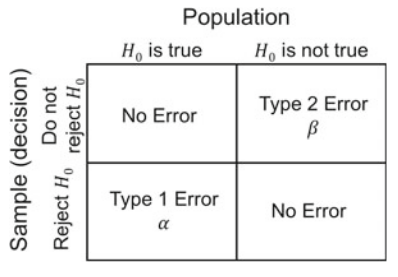
\includegraphics[
        width=\linewidth,
        height=5cm,
        keepaspectratio,
    ]{images/statistics/hypothesis-testing-errors.png}
    \caption{
        Types of errors in hypothesis testing
        \cite{statistics/book/Statistics-for-Data-Scientists/Maurits-Kaptein}
    }
\end{figure}

    \item 4 situations:
    \begin{enumerate}
        \item {[\textbf{true positive}]} we do not reject $H_0$ when $H_0$ is true in the population
        \hfill \cite{statistics/book/Statistics-for-Data-Scientists/Maurits-Kaptein}

        \item {[\textbf{true negative}]} we reject $H_0 $, and subsequently accept $H_a $, when $H_a$ is true in the population
        \hfill \cite{statistics/book/Statistics-for-Data-Scientists/Maurits-Kaptein}

        \item {[\textbf{false positive}]} we reject $H_0$ while in reality it is true, aka false positive or type 1 error.
        The probability of a type 1 error is associated with the level $\alpha$.
        The $\alpha$ is used as a maximal allowable type 1 error for a decision rule.
        \hfill \cite{statistics/book/Statistics-for-Data-Scientists/Maurits-Kaptein}

        \item {[\textbf{false negative}]} we do not reject $H_0$ , while in actuality $H_a$ is true, aka type 2 error.
        The probability of a type 2 error is associated with the level $\beta$.
        The value $\beta$ is used a maximal allowable type 2 error.
        One minus the type 2 error ($1-\beta$) is called the \textbf{power} of the binary decision rule.
        It indicates how likely the null hypothesis is rejected when the alternative hypothesis is true.
        \hfill \cite{statistics/book/Statistics-for-Data-Scientists/Maurits-Kaptein}
    \end{enumerate}

    \item it is easy to create a decision procedure that has a type 1 error probability equal to zero:
    if we simply never reject $H_0$ —in this case basically we state that there is never sufficient evidence to reject $H_0$ —we will never make a type 1 error.
    While this decision procedure does control the type 1 error, it is clearly not very useful, as the power of this decision rule is zero: we never accept the alternative hypothesis when it is true.
    \hfill \cite{statistics/book/Statistics-for-Data-Scientists/Maurits-Kaptein}

    \item the procedure of hypothesis testing aims to be less conservative (e.g., it will reject the null hypothesis sometimes but not too often when it would be true).
    \hfill \cite{statistics/book/Statistics-for-Data-Scientists/Maurits-Kaptein}

    \item \textbf{One tailed test}: Test statistics falls into one specified tail of its sampling distribution
    \hfill \cite{ctl.unm.edu/assets/docs/resources/hypothesis-testing-sheet.pdf}

    \item \textbf{Two tailed test}: Test statistics can falling into either tail of its sampling distribution
    \hfill \cite{ctl.unm.edu/assets/docs/resources/hypothesis-testing-sheet.pdf}

    \item Steps to Significance Testing:
    \hfill \cite{ctl.unm.edu/assets/docs/resources/hypothesis-testing-sheet.pdf}
    \begin{enumerate}
        \item Define $H_0$ and $H_a$
        \hfill \cite{ctl.unm.edu/assets/docs/resources/hypothesis-testing-sheet.pdf}

        \item Identify test, $\alpha$, find critical value, test statistics
        \hfill \cite{ctl.unm.edu/assets/docs/resources/hypothesis-testing-sheet.pdf}

        \item Construct acceptance/rejection regions
        \hfill \cite{ctl.unm.edu/assets/docs/resources/hypothesis-testing-sheet.pdf}

        \item Calculate test statistics
        \hfill \cite{ctl.unm.edu/assets/docs/resources/hypothesis-testing-sheet.pdf}

        \begin{enumerate}
            \item Critical value approach: Determine critical region
            \hfill \cite{ctl.unm.edu/assets/docs/resources/hypothesis-testing-sheet.pdf}

            \item p-value approach: Calculate p-value
            \hfill \cite{ctl.unm.edu/assets/docs/resources/hypothesis-testing-sheet.pdf}
        \end{enumerate}

        \item Retain or reject the hypothesis
        \hfill \cite{ctl.unm.edu/assets/docs/resources/hypothesis-testing-sheet.pdf}
    \end{enumerate}

    \item \textbf{Choosing a Statistical Test}:

\begin{figure}[H]
    \centering
    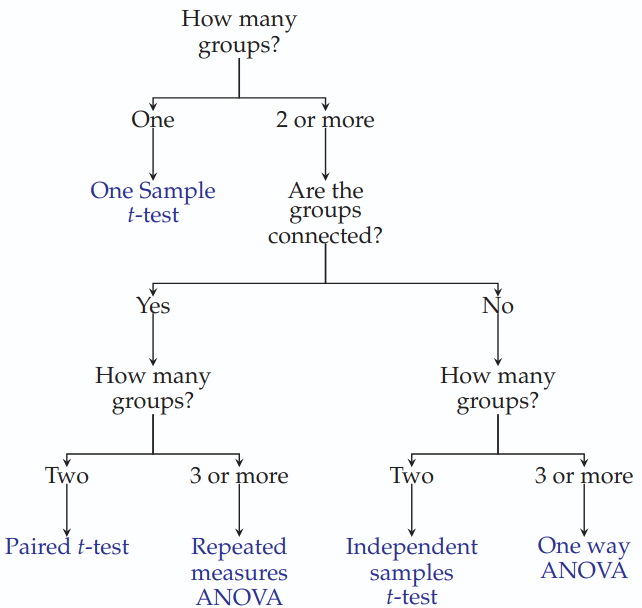
\includegraphics[
        width=\linewidth,
        height=7cm,
        keepaspectratio,
    ]{images/statistics/hypothesis-testing-desicion-tree.png}
    \caption{
        Choosing a Statistical Test: Decision Tree
        \cite{ctl.unm.edu/assets/docs/resources/hypothesis-testing-sheet.pdf}
    }
\end{figure}

    \begin{enumerate}
        \item Categorical Data: Use Chi Square
        \hfill \cite{ctl.unm.edu/assets/docs/resources/hypothesis-testing-sheet.pdf}

        \item Sample size ($n$):
        \begin{enumerate}
            \item $n < 30$ and Population Variance is unknown - t-test
            \hfill \cite{ctl.unm.edu/assets/docs/resources/hypothesis-testing-sheet.pdf}

            \item $n < 30$ and Population Variance is known - z-test
            \hfill \cite{ctl.unm.edu/assets/docs/resources/hypothesis-testing-sheet.pdf}

            \item $n > 30$ - z-test or t-test
            \hfill \cite{ctl.unm.edu/assets/docs/resources/hypothesis-testing-sheet.pdf}
        \end{enumerate}
    \end{enumerate}
\end{enumerate}



\subsection{The One-Sided $z$-Test for a Single Mean}

\begin{enumerate}
    \item hypothesis on the population mean: $H_0 : \mu( f ) \leq \mu_0$ versus $H_a : \mu( f ) > \mu_0 $.
    \hfill \cite{statistics/book/Statistics-for-Data-Scientists/Maurits-Kaptein}

    \item we assume that the sample is large enough to be able to use the normal distribution function as an approximation to the distribution function of the statistic that we are using to make a decision about the null hypothesis
    \hfill \cite{statistics/book/Statistics-for-Data-Scientists/Maurits-Kaptein}

    \item Let’s assume that we have collected a random sample $Y_1 , Y_2, \cdots , Y_n$ from the population.
    We may estimate the population mean $\mu ( f )$ with the sample average $\bar{Y}$ .
    \hfill \cite{statistics/book/Statistics-for-Data-Scientists/Maurits-Kaptein}

    \item when $\bar{Y}$ is smaller or equal to $\mu_0$ the random variable $\bar{Y}$ seems to be in line with the null hypothesis $H_0 : \mu( f ) \leq \mu_0$ .
    In other words, there is no evidence that the \textbf{null hypothesis is false}.
    \hfill \cite{statistics/book/Statistics-for-Data-Scientists/Maurits-Kaptein}

    \item Although the random variable does not suggest any conflict with the null hypothesis $H_0 : \mu( f ) \leq \mu_0 $, it \textbf{does not guarantee} that $\mu( f ) \leq \mu_0$ either.
    \hfill \cite{statistics/book/Statistics-for-Data-Scientists/Maurits-Kaptein}

    \item If the population mean $\mu( f )$ were somewhat larger than $\mu_0 $, it might not be completely unlikely to observe a sample average still below $\mu_0$ due to the sampling (a type 2 error).
    \hfill \cite{statistics/book/Statistics-for-Data-Scientists/Maurits-Kaptein}

    \item When $\bar{Y}$ is larger than $\mu_0 $, we might start to believe that the null hypothesis is incorrect.
    However, when $\bar{Y}$ is just a little higher than $\mu_0$ this might not be very unlikely either, even when $\mu( f ) \leq \mu_0$ .
    \hfill \cite{statistics/book/Statistics-for-Data-Scientists/Maurits-Kaptein}

    \item For instance, for any symmetric $f$ at $\mu( f ) = \mu_0 $, the probability that $\bar{Y}$ is larger than $\mu_0$ is equal to $0.5$.
    Only when the sample average $\bar{Y}$ is substantially larger—thus when there is sufficient evidence—than $\bar{Y}$ would we start to indicate that the null hypothesis $H_0 : \mu( f ) \leq \mu_0$ is unlikely to be true (although a type 1 error could be made here).
    \hfill \cite{statistics/book/Statistics-for-Data-Scientists/Maurits-Kaptein}

    \item we want to find a criterion for the average $\bar{Y}$ such that the average can only be larger than this criterion with a probability that is at most equal to $\alpha$ when the null hypothesis is true. 
    If we assume that this criterion is equal to $\mu_0 + \delta$, with $\delta > 0$, then the probability that $\bar{Y}$ is larger than $\mu_0 + \delta$ is given by
    \hfill \cite{statistics/book/Statistics-for-Data-Scientists/Maurits-Kaptein}
    \\[0.3cm]
    .\hfill
    $
        P( \bar{Y} > \mu _0 + \delta)
        = P\dParenBrac{\dfrac{ ( \bar{Y} - \mu ( f ))}{\sigma( f )/\sqrt{n}} > \dfrac{\mu _0 - \mu ( f ) + \delta}{\sigma/\sqrt{n}}}
        \approx 1 - \Phi\dParenBrac{\dfrac{\mu _0 - \mu ( f ) + \delta}{\sigma( f )/\sqrt{n}}}
    $
    \hfill \cite{statistics/book/Statistics-for-Data-Scientists/Maurits-Kaptein}
    \\[0.3cm]
    where $\Phi$ is the standard normal PDF.
    \hfill \cite{statistics/book/Statistics-for-Data-Scientists/Maurits-Kaptein}

    \item Under the null hypothesis $H_0 : \mu( f ) \leq \mu_0$ this probability is the type 1 error and it is maximized when $\mu( f ) = \mu_0$ .
    \hfill \cite{statistics/book/Statistics-for-Data-Scientists/Maurits-Kaptein}

    \item if we deliberately set $\mu( f ) = \mu_0$ to maximize the type 1 error, the probability $P ( \bar{Y} > \mu_0 + \delta)$ is given by $1 - \Phi(\delta\sqrt{n}/\sigma)$.
    \hfill \cite{statistics/book/Statistics-for-Data-Scientists/Maurits-Kaptein}

    \item When we choose $\delta$ equal to $\delta = \dfrac{z_{1-\alpha} \sigma( f )}{\sqrt{n}}$, the probability becomes $P ( \bar{Y} > \mu_0 + \delta) \approx \alpha$. 
    When $\bar{Y} > \mu_0 + \dfrac{z_{1 - \alpha} \sigma( f )}{\sqrt{n}}$ the probability of rejecting the null hypothesis is at most $\alpha$—and hence we have defined sufficient evidence by the criterion $\mu0 + \dfrac{z_{1 - \alpha} \sigma( f )}{\sqrt{n}}$ for the null hypothesis $H_0 : \mu( f ) \leq \mu_0$ using the statistic $\bar{Y} $. 
    \hfill \cite{statistics/book/Statistics-for-Data-Scientists/Maurits-Kaptein}

    \item The null hypothesis could still be true, but that it is just bad luck to have observed such an unlikely large average under the null hypothesis.
    However, we know that this probability of having bad luck is less than or equal to $\alpha$ and therefore we accept making this potential type 1 error.
    \hfill \cite{statistics/book/Statistics-for-Data-Scientists/Maurits-Kaptein}

    \item we cannot use the criterion ¯$Y > μ_0 + \dfrac{z_{1−α} σ( f )}{\sqrt{n}}$ directly, as it depends on the population standard deviation $σ( f )$, which is generally not known.
    We could estimate $σ( f )$ using sample standard deviation $S = \sqrt{\dfrac{1}{n−1} \dsum^n_{i=1} (Y_i − ¯Y )^2}$
    \hfill \cite{statistics/book/Statistics-for-Data-Scientists/Maurits-Kaptein}

    \item If the sample size is large enough, the probability $P\dParenBrac{¯Y > μ_0 + \dfrac{z_{1−α} S}{\sqrt{n}}}$ would still be close to $α$. 
    When the sample size is large enough, we may reject the null hypothesis in practice when $¯Y > μ0 + \dfrac{z_{1−α} S}{\sqrt{n}}$ or in other words when the \textbf{asymptotic test statistic} $T_n = \dfrac{¯Y − μ_0}{S/√n}$ is larger than $z_{1−α}$.
    \hfill \cite{statistics/book/Statistics-for-Data-Scientists/Maurits-Kaptein}

    \item 
    \hfill \cite{statistics/book/Statistics-for-Data-Scientists/Maurits-Kaptein}
\end{enumerate}

































